\begin{center}\small
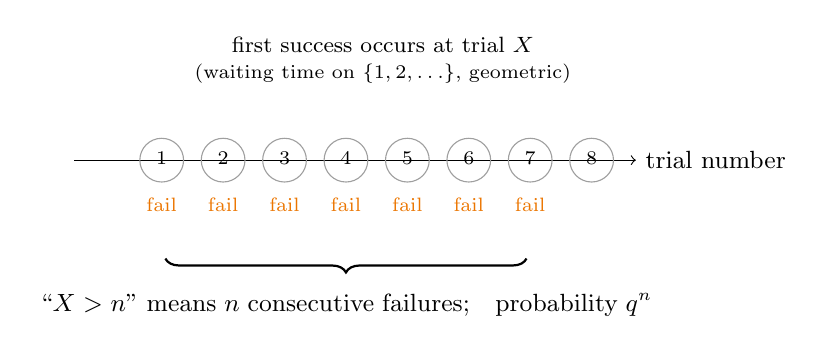
\begin{tikzpicture}[x=0.78cm,y=1cm]

  % Explain the picture above the numbered trials (nothing overlaps circles or ``fail'' row)
  \node[
    align=center,
    font=\footnotesize,
  ] at (4.6, 1.62)
    {first success occurs at trial $X$\\
     {\scriptsize (waiting time on $\{1,2,\ldots\}$, geometric)}};

  \draw[->] (-0.42, 0.35) -- (8.72, 0.35)
    node[right, font=\small] {trial number};

  % Trial markers — row $y = 0.35$
  \foreach \t in {1,...,8}{
    \node[
      circle,
      draw=gray!75,
      minimum size=1.58em,
      inner sep=0pt,
      font=\scriptsize,
    ] at (\t, 0.35) {\strut$\t$};
  }

  % Outcomes row: one ``fail'' word per column (trials $1$--$7$)
  \foreach \t in {1,...,7}{
    \node[
      anchor=north,
      font=\scriptsize,
      text=orange!92!black,
    ] at (\t, 0.02) {\strut fail};
  }

  % Brace spanning trials $1,\ldots,n$ illustrating $q^n$
  \draw[thick, decorate, decoration={brace, mirror, amplitude=5pt}]
    (1.06, -0.90) -- (6.94, -0.90)
    node[
      midway,
      below=9pt,
      font=\footnotesize,
      align=center,
      text width=7.85cm,
    ]
    {\small ``$X>n$'' means $n$ consecutive failures;\quad probability $q^n$};

\end{tikzpicture}\\[2.55em]

\noindent\footnotesize\textit{Geometric waiting picture: memorylessness compares $P(X>n+k\mid X>n)$ with fresh starts.}
\end{center}
